\subsubsection{Quản lý biểu mẫu}

    Module Biểu mẫu cung cấp các chức năng quản lý và sử dụng biểu mẫu động cho các hoạt động của đoàn hội, bao gồm 2 chức năng chính:

    \begin{enumerate}
        \item \textbf{Quản lý biểu mẫu:} Tải lên file Word template, cấu hình trường dữ liệu động, quản lý danh sách biểu mẫu.
        \item \textbf{Điền thông tin vào biểu mẫu:} Sinh viên/Thành viên điền biểu mẫu, hệ thống tự động sinh file Word/PDF từ template.
    \end{enumerate}

    Module hỗ trợ parse file Word template với các placeholder động, cho phép tạo biểu mẫu tùy chỉnh mà không cần code.

    % UC8.1 - Quản lý biểu mẫu
    \newpage
    \begin{figure}[H]
        \centering
        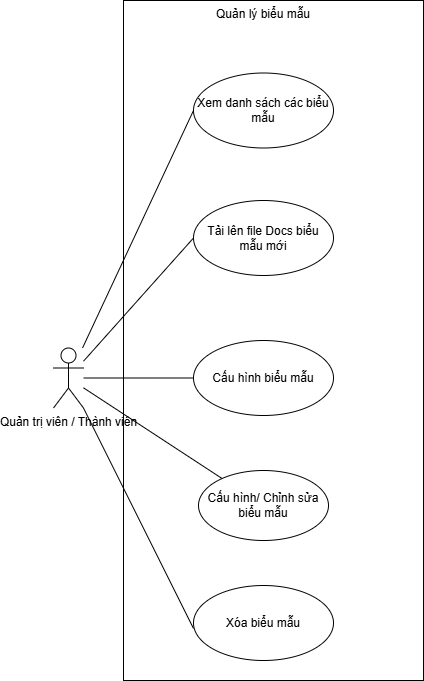
\includegraphics[width=0.7\linewidth]{Images/use-case-diagram/UC08_01_quan_ly_bieu_mau.png}
        \vspace{0.3em}
        \captionsetup{skip=8pt}
        \caption{UC8.1 - Quản lý biểu mẫu}
        \label{fig:uc08-01}
    \end{figure}

    \newpage
    \begin{table}[H]
    \renewcommand{\arraystretch}{1.3}
    \begin{tabular}{|m{0.25\textwidth}|m{0.75\textwidth}|}
    \hline
    \textbf{Use Case Name} 
    & \textbf{UC8.1. Quản lý biểu mẫu} \\ \hline

\textbf{Actors} 
& Quản trị viên, Người dùng \\ \hline

\textbf{Description}
    & Use case này cho phép quản lý biểu mẫu Word động trong hệ thống. Bao gồm:
    \begin{itemize}
        \item Xem danh sách biểu mẫu
        \item Tải lên file Word template mới
        \item Cấu hình trường dữ liệu động (placeholder)
        \item Chỉnh sửa cấu hình biểu mẫu
        \item Xóa biểu mẫu
    \end{itemize}
    \\ \hline

    \textbf{Trigger} 
    & Quản trị viên/Người dùng muốn tạo hoặc quản lý biểu mẫu cho các hoạt động.
    \\ \hline

    \textbf{Pre-Conditions} 
    & \begin{itemize}
        \item Người dùng đã đăng nhập
        \item Có quyền quản lý biểu mẫu
    \end{itemize}
    \\ \hline

    \textbf{Post-Conditions} 
    & \begin{itemize}
        \item Biểu mẫu được tạo mới, cấu hình hoặc xóa trong hệ thống
        \item File template được lưu trên S3
        \item Cấu hình trường được lưu trong database
    \end{itemize}
    \\ \hline

    \textbf{Normal Flow} 
    & \textbf{Tải lên biểu mẫu mới:}
    \begin{enumerate}
        \item Người dùng click "Tạo biểu mẫu", nhập tên và tải lên file Word
        \item Hệ thống parse file, trích xuất các placeholder ({{tên\_trường}})
        \item Hiển thị danh sách placeholder tìm thấy
        \item Người dùng cấu hình từng placeholder: loại dữ liệu, nhãn hiển thị, bắt buộc/tùy chọn
        \item Lưu template lên S3 và cấu hình vào database
    \end{enumerate}

    \textbf{Chỉnh sửa cấu hình:}
    \begin{enumerate}
        \item Người dùng click "Cấu hình" trên biểu mẫu
        \item Hệ thống hiển thị danh sách placeholder và cấu hình hiện tại
        \item Người dùng chỉnh sửa cấu hình trường
        \item Cập nhật cấu hình vào database
    \end{enumerate}

    \textbf{Xóa biểu mẫu:}
    \begin{enumerate}
        \item Người dùng click "Xóa"
        \item Hệ thống kiểm tra: nếu có bản ghi đã nộp thì không cho xóa
        \item Nếu không có: xóa file trên S3 và xóa mềm trong database
    \end{enumerate}
    \\ \hline
    \end{tabular}
    \end{table}

    \newpage
    \begin{table}[H]
    \renewcommand{\arraystretch}{1.3}
    \begin{tabular}{|m{0.25\textwidth}|m{0.75\textwidth}|}
    \hline
    \textbf{Alternative Flow} 
    & \textbf{Tải lên:}
    \begin{itemize}
        \item \textbf{2a.} File không phải .docx: Hiển thị "Chỉ hỗ trợ file .docx", quay lại bước 1
        \item \textbf{2b.} File > 5MB: Hiển thị "File quá lớn, tối đa 5MB", quay lại bước 1
        \item \textbf{3a.} Không tìm thấy placeholder: Hiển thị cảnh báo "Template không có trường động", vẫn cho lưu
        \item \textbf{5a.} Lỗi tải lên S3: Hiển thị "Lỗi khi lưu file, vui lòng thử lại"
    \end{itemize}

    \textbf{Chỉnh sửa:}
    \begin{itemize}
        \item \textbf{2a.} Biểu mẫu không tồn tại: Hiển thị lỗi không tìm thấy
    \end{itemize}

    \textbf{Xóa:}
    \begin{itemize}
        \item \textbf{2a.} Có bản ghi đã nộp: Hiển thị "Không thể xóa biểu mẫu đã có người nộp", không cho xóa
        \item \textbf{3a.} Người dùng click "Hủy": Đóng hộp thoại, không xóa
    \end{itemize}
    \\ \hline

    \textbf{Exception} 
    & \begin{itemize}
        \item Lỗi phân tích file Word: Hiển thị "File không đúng định dạng hoặc bị lỗi"
        \item Lỗi kết nối S3: Hiển thị "Lỗi lưu trữ, vui lòng thử lại sau"
        \item Lỗi cơ sở dữ liệu: Hiển thị "Không thể lưu cấu hình, vui lòng thử lại"
    \end{itemize}
    \\ \hline
    \end{tabular}
    \caption{Bảng mô tả Use Case UC8.1 - Quản lý biểu mẫu}
    \end{table}

    % ========================================
    % UC8.2 - Điền thông tin vào biểu mẫu
    \newpage
    \begin{figure}[H]
        \centering
        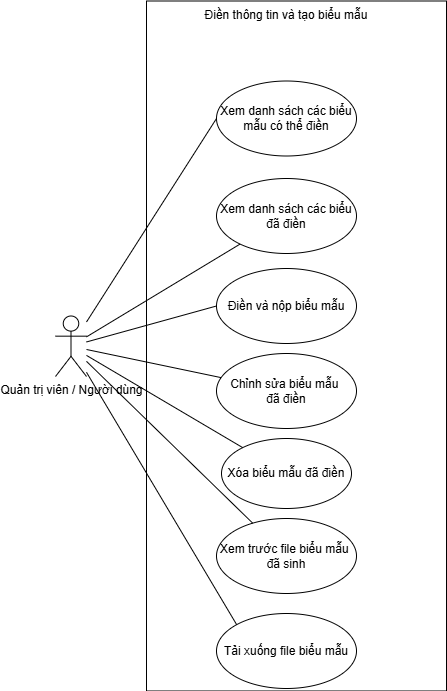
\includegraphics[width=0.8\linewidth]{Images/use-case-diagram/UC08_02_dien_bieu_mau.png}
        \vspace{0.3em}
        \captionsetup{skip=8pt}
        \caption{UC8.2 - Điền thông tin vào biểu mẫu}
        \label{fig:uc08-02}
    \end{figure}

    \newpage
    \begin{table}[H]
    \renewcommand{\arraystretch}{1.3}
    \begin{tabular}{|m{0.25\textwidth}|m{0.75\textwidth}|}
    \hline
    \textbf{Use Case Name} 
    & \textbf{UC8.2. Điền thông tin vào biểu mẫu} \\ \hline

\textbf{Actors} 
& Quản trị viên, Người dùng, Thành viên \\ \hline

\textbf{Description} 
    & Use case này cho phép người dùng điền thông tin vào biểu mẫu và hệ thống tự động sinh file Word/PDF. Bao gồm:
    \begin{itemize}
        \item Xem danh sách biểu mẫu có thể điền
        \item Xem danh sách biểu mẫu đã điền
        \item Điền và nộp biểu mẫu mới
        \item Chỉnh sửa biểu mẫu đã nộp
        \item Xóa biểu mẫu đã nộp
        \item Xem trước file đã sinh
        \item Tải xuống file Word/PDF
    \end{itemize}
    \\ \hline

    \textbf{Trigger} 
    & Người dùng muốn điền biểu mẫu hoặc quản lý các biểu mẫu đã nộp.
    \\ \hline

    \textbf{Pre-Conditions} 
    & \begin{itemize}
        \item Người dùng đã đăng nhập
        \item Có ít nhất 1 biểu mẫu trong hệ thống
    \end{itemize}
    \\ \hline

    \textbf{Post-Conditions} 
    & \begin{itemize}
        \item Bản ghi nộp được tạo/cập nhật trong database
        \item File Word/PDF được sinh và lưu trên S3
        \item Người dùng có thể tải xuống file đã sinh
    \end{itemize}
    \\ \hline

    \textbf{Normal Flow} 
    & \textbf{Điền biểu mẫu mới:}
    \begin{enumerate}
        \item Người dùng chọn biểu mẫu, click "Điền biểu mẫu"
        \item Hệ thống hiển thị form với các trường từ cấu hình
        \item Người dùng điền thông tin và click "Nộp"
        \item Hệ thống validate, thay thế placeholder trong template, sinh file Word/PDF
        \item Lưu bản ghi nộp và file lên S3, hiển thị "Nộp thành công"
    \end{enumerate}

    \textbf{Chỉnh sửa bản ghi đã nộp:}
    \begin{enumerate}
        \item Người dùng click "Chỉnh sửa" trên bản ghi đã nộp
        \item Hệ thống hiển thị form với dữ liệu cũ
        \item Người dùng sửa thông tin và click "Cập nhật"
        \item Sinh lại file mới, cập nhật bản ghi nộp
    \end{enumerate}

    \textbf{Xem trước/Tải xuống:}
    \begin{enumerate}
        \item Người dùng click "Xem trước" hoặc "Tải xuống"
        \item Hệ thống lấy file từ S3
        \item Xem trước trong browser hoặc tải xuống file
    \end{enumerate}
    \\ \hline
    \end{tabular}
    \end{table}

    \newpage
    \begin{table}[H]
    \renewcommand{\arraystretch}{1.3}
    \begin{tabular}{|m{0.25\textwidth}|m{0.75\textwidth}|}
    \hline
    \textbf{Alternative Flow} 
    & \textbf{Điền biểu mẫu:}
    \begin{itemize}
        \item \textbf{4a.} Trường bắt buộc bỏ trống: Hiển thị lỗi validate, quay lại bước 3
        \item \textbf{4b.} Dữ liệu không đúng định dạng: Hiển thị lỗi cụ thể, quay lại bước 3
        \item \textbf{5a.} Lỗi sinh file: Hiển thị "Không thể tạo file, vui lòng thử lại"
    \end{itemize}

    \textbf{Chỉnh sửa:}
    \begin{itemize}
        \item \textbf{1a.} Bản ghi nộp không tồn tại: Hiển thị lỗi không tìm thấy
        \item \textbf{1b.} Không có quyền sửa (không phải người nộp): Hiển thị "Bạn không có quyền"
    \end{itemize}

    \textbf{Xem trước/Tải xuống:}
    \begin{itemize}
        \item \textbf{2a.} File không tồn tại trên S3: Sinh lại file từ dữ liệu đã nộp
        \item \textbf{2b.} Lỗi kết nối S3: Hiển thị "Không thể tải file, vui lòng thử lại"
    \end{itemize}
    \\ \hline

    \textbf{Exception} 
    & \begin{itemize}
        \item Template bị xóa: Hiển thị "Biểu mẫu không còn tồn tại"
        \item Lỗi xử lý template: Hiển thị "Lỗi xử lý biểu mẫu, vui lòng liên hệ quản trị viên"
        \item Lỗi tải lên S3: Hiển thị "Không thể lưu file, vui lòng thử lại"
    \end{itemize}
    \\ \hline
    \end{tabular}
    \caption{Bảng mô tả Use Case UC8.2 - Điền thông tin vào biểu mẫu}
    \end{table}
